\documentclass{ttithesis}

\usepackage{amsmath}
\usepackage{graphicx}
\usepackage{scrextend}
\usepackage{setspace}
\usepackage{color}


\title{文間及びカテゴリ間の関係性を捉えた\\レーティング予測}
\author{12056\hspace{16ex}外山洋太}
\date{平成28年 2月}
\laboratory{知能数理研究室}



\begin{document}

\section{序論}

企業において商品の評判分析のためのレビューの評判分類は重要な問題である。
何万件という大量のレビューデータを人手で処理することは難しく、
計算機による自動化が望まれる。
その中で商品を複数のカテゴリにおいて分類をする問題がある。
カテゴリとは、宿泊施設のレビューを例にすると、サービス、立地、食事等の
レーティングが付けられる各項目のことである。
この問題に関する従来手法\cite{fujitani15}は、文間の関係性を考慮しておらず、
カテゴリ間については考慮しているものの深い関係性を捉えることができていない。

近年、その評判分類において、ニューラルネットワークを用いた手法が
提案されており、従来の手法を上回る分類精度を達成している。
ニューラルネットワークを分類問題に用いることの利点の一つは
層の数を増やすことによって
入力となる特徴量の深い意味を捉えることができることである。
多カテゴリの分類問題に適用すれば、
カテゴリ間の関係性を捉えた分類が実現できる。
さらに、文毎の特徴量を入力とすれば文間の関係性も捉えることができる。

文や文章の特徴量としては、パラグラフベクトル\cite{quoc14}が分類問題に対して
優れていることが示されている。

以上より、本研究では、複数カテゴリにおける評判分類について、
パラグラフベクトルとCNNを用いて文間及びカテゴリ間の関係性を捉えた分類を実現し、
従来手法から分類精度を向上させることを目的とした。

提案手法は、パラグラフベクトルによって生成された各レビューの特徴量を
ニューラルネットワークの分類器において分類しレーティング予測を行う。
特徴量としては、各レビューの文書ベクトルに加え、各レビュー内の文ベクトルの
重み付け平均を用いた。
分類器は全結合ニューラルネットワークによって構成されており、
文間及びカテゴリ間の関係性を捉えた分類を行う。

実験において、提案手法は従来手法\cite{fujitani15}に対して2pp以上上回る精度を
示した。
正解ラベルと予測したラベルの差を元にした評価基準でも、多くのカテゴリにおいて
従来手法\cite{fujitani15}を上回る結果を示した。
また、実験により、パラグラフベクトルが文書と文について適用された場合、
文書ベクトルと文ベクトルは異なる特徴を捉えていることが示された。



\section{関連研究}

\subsection{隠れ状態を用いたホテルレビューのレーティング予測}

藤谷ら\cite{fujitani15}は複数のカテゴリにおける評判分類問題に対して、
レビュー内の各文毎に予測した隠れレーティングから
レビュー全体のレーティングを予測する手法を提案している。
文毎のレーティングからレビュー全体のレーティングを予測する際の
カテゴリ間の繋がりを手動で変化させカテゴリ間の関係性を考慮している。

実験結果より、各文毎に隠れレーティングを予測することによって
分類精度が向上すること、
また、カテゴリ間の繋がりによって分類精度が変化することが示されている。


\subsection{パラグラフベクトル}

パラグラフベクトルは、文や文章といった大きな単位の言語表現の意味表現を
学習する手法である。これは、Continuous Bag Of Words
(CBOW)という単語の意味表現の 学習手法を応用した手法である。

以下に具体的なアルゴリズムを示す。
ここでは文章の意味表現を学習する場合について考える。
学習の概略を図\ref{fig:ParagraphVector}に示す。

まず、意味表現を学習する対象となる文に含まれる単語を
初めから一つずつ読んでいく。
その際、以下の式1に示す目的関数を最大化するように各パラメータの学習を行う。

\begin{gather}
  L = \frac{1}{T} \sum^{T - k}_{t = k} \log p(w_t | w_{t-k}, ..., w_{t+k}) \\
  p(w_t | w_{t-k}, ..., w_{t+k}) = \frac{e^{y_{w_t}}}{\sum_i e^{y_i}} \\
  y = b + Uh(w_{t-k}, ..., w_{t+k}, d; W, D)
\end{gather}

ここで、$d$は文、$w_i$は単語、$W$は全ての単語の分散表現を表す行列、
$D$は学習している全ての文章の分散表現を表す行列である。
$k$は片側のウィンドウサイズ、
$T$は現在の文章に含まれる単語数である。
$y$は現在の単語とウィンドウ内のその周りの単語及び現在の文章から導出される
対数確率である。 この値は、現在の単語とその文脈との類似度を表す。
$p$はsoftmax関数により正規化された、文脈から現在の単語が導かれることの
尤度である。

また、学習効率を高めるために、ネガティブサンプリングを行う場合がある、
ネガティブサンプリングとは、文脈外の単語をデータセットにおける出現確率で
サンプリングし、それらと文脈の意味が遠ざかるように$y$の式を決め
学習する手法である。

これにより、Bag Of Words (BOW)と異なり、
単語の並び順を考慮した文や文章の分散表現を生成することができる。

\begin{figure}
  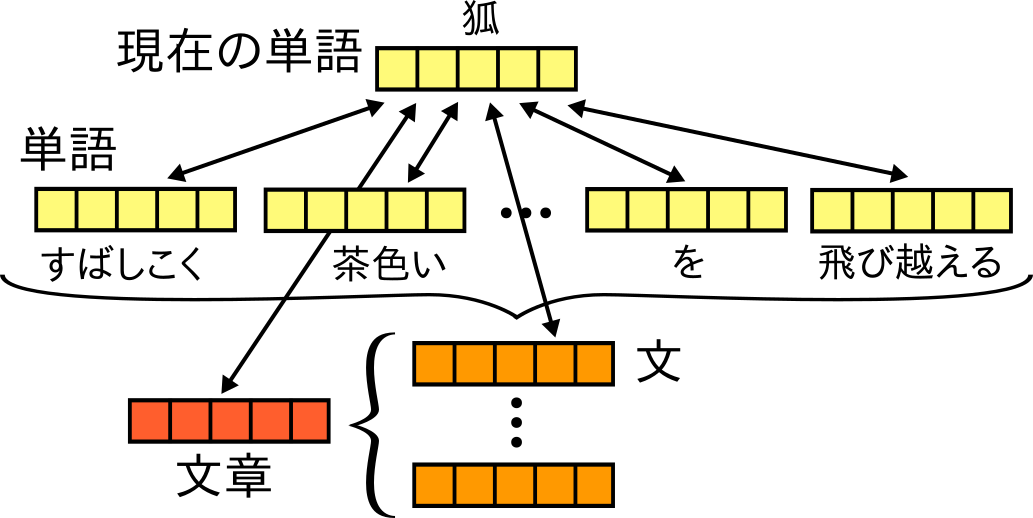
\includegraphics{fig/dvsvwv.png}
  \caption{文書及び文ベクトルの学習の概略}
  \label{fig:ParagraphVector}
\end{figure}


\subsection{ニューラルネットワークを用いた評判分析}

 ニューラルネットワークを用いた評判分析の手法が、Nalら\cite{nal14}、
Rieら\cite{rie14}、Duyuら\cite{duyu15}等によって提案されている。

 これらの方法は、まず、単語の分散表現から畳み込みニューラルネットワークを
用いて単語同士の関係を捉えた特徴量を抽出する。その後、そこから得られた
文書あるいは文全体の特徴量を全結合ニューラルネットワークの入力とし
多値または二値分類を行う。
また、これらの手法はニューラルネットワークのモデルの中にパラメータとして
単語の分散表現を取り込んでいる。これにより、特定の分類問題に対して
それらを微調整することが可能になる。



\section{提案手法}

提案手法では、パラグラフベクトルによってレビュー内の各文及び文章の分散表現を
生成し、それらをニューラルネットワークの入力として分類を行う。
以下にその基礎となるアイデアと具体的なアルゴリズムを示す。


\subsection{アイデア}

先行研究\cite{fujitani15}の実験結果から、
レビュー内の各文の特徴量を元にレビューの分類を行うことが
分類精度の向上に有効であると考えられる。
また、カテゴリ間の繋がりの変化が分類精度に影響していることから、
これをパラメータとして機械学習のモデルに組み込めば
分類精度を向上させることができると考えられる。

さらに、レビュー内の各文毎に分散表現を生成し分類器の入力とすることで、
その順序を考慮した学習を行う。
これにより、レビュー内の文の位置関係がレーティング予測時に利用できると
考えられる。
以下に、文の位置関係が重要となる例を示す。
2つ目の例は、1つ目の例の1つ目の文と3つ目の文を入れ替えたものである。

\begin{addmargin}{8ex}
  \vspace{1em}
  \setstretch{1}
  食事は本格的で新鮮な食材が使われており美味しかった。
  しかし、それよりも嬉しかったことがある。
  それは、部屋からの海の眺めが素晴らしかったことである。
  これには子供も喜んでいた。
\end{addmargin}

\begin{addmargin}{8ex}
  \vspace{1em}
  \setstretch{1}
  \textcolor{red}{それは、部屋からの海の眺めが素晴らしかったことである。}
  しかし、それよりも嬉しかったことがある。
  \textcolor{red}{食事は本格的で新鮮な食材が使われており美味しかった。}
  これには子供も喜んでいた。
\end{addmargin}

1つ目の例では、4つ目の文が直前の立地が良かったという文の
意味を補完しているのに対し、
2つ目の例では、食事が良かったという文の意味を補完している。
このように、文の位置関係によってどの文がどの文と強く関連しているかが
変化する。それによって推定すべきレビュー全体のレーティングも変わると
考えられる。よって、文の位置関係を考慮することは重要である。

しかし、個々のレビューに対して全ての文ベクトルを用いるのには、問題がある。
なぜならば、各レビュー内の文の数はまちまちであり、データ上単純な行列として
表せないためである。
これは、ミニバッチ方式の訓練を難しくし、実行時間の増加に繋がる。
この問題に対処するため、本手法では各レビュー内の文ベクトルに対して
重み付け平均を行った。これにより、全てのレビューで文ベクトルの数が揃い、
複数レビュー内の複数の文ベクトルをまとめて3次元行列として表すことができる。
つまり、ミニバッチ方式の計算が容易となる。

分類器はニューラルネットワークを用いて構成することによって、文の位置関係と
カテゴリ間の関係を同時に捉えた分類を行う。従来手法\cite{nal14}や
\cite{rie14}、\cite{duyu15}では、単語ベクトルに対して
畳込みニューラルネットワークが用いられている。
しかし、提案手法においては、畳み込みニューラルネットワークより
全結合ニューラルネットワークを用いた方が精度が高かったため、
分類器には後者のみを用いた。


\subsection{アルゴリズム}

実際のアルゴリズム全体の流れを説明する。
図\ref{fig:MyAlgorithm}にアルゴリズム全体の概略を示す。

\begin{figure}
  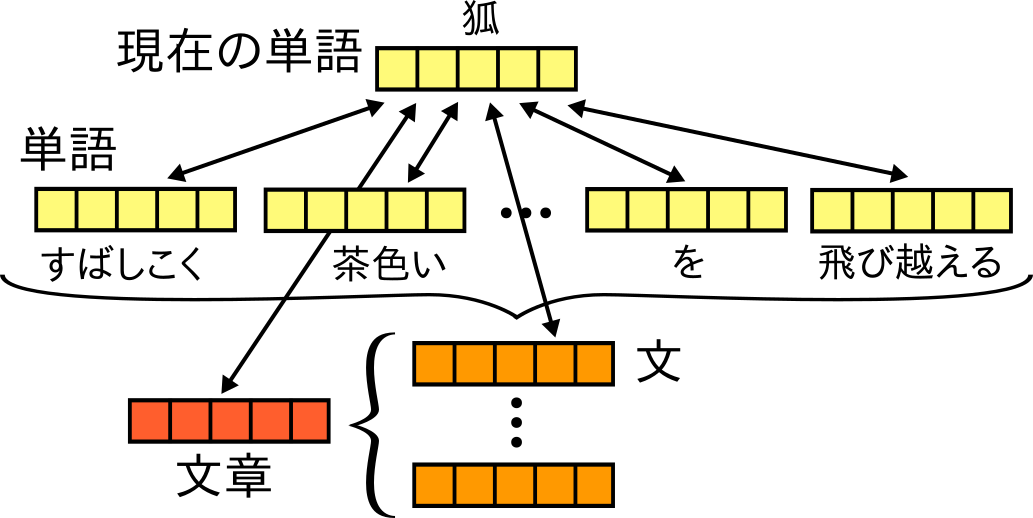
\includegraphics{fig/dvsvwv.png}
  \caption{提案手法におけるアルゴリズムの概略}
  \label{fig:MyAlgorithm}
\end{figure}

初めに、パラグラフベクトルを用いて、
各レビューの文書ベクトルとそれに含まれる各文のベクトルを生成する。
文書ベクトルと文ベクトルについては別々のモデルを学習させ生成する。

次に、各レビュー内の全ての文ベクトルに対して重み付け平均を行い、
圧縮された文ベクトルを生成する。
この過程により、各レビューで疎らだった文の数が統一される。
以下に重み付け平均を行う関数を示す。

\begin{gather}
t_{i_{sect}} = \sum_{i_{sent}} \frac{\mathbf{w}(x_{i_{sect}}(i_{sent})}
                                    {|\mathbf{w}(x_{i_{sect}}(i_{sent}))|}
                               s_{i_{sent}} \\
x_{i_{sect}}(i_{sent}) = \frac{i_{sent} - i_{sect}}{\#sections} \\
\mathbf{w}(x) = (w_{1}(x), w_{2}(x), ..., w_{i_{sect}}(x),
                 ..., w_{\#sentences}(x)) \\
w(x) = \frac{1}{2} (\cos(\pi|x|) + 1) \hspace{8ex} \text{if $|x| <= 1$}
\end{gather}

ここで、$i_{sent}$はレビュー内の文のインデックス、
$\#sections$は重み付け平均された後の文ベクトルの数、
$i_{sect}$は重み付け平均された後の文ベクトルのインデックスである。
$s_{i_{sent}}$は文ベクトル、$t_{i_{sect}}$は圧縮された後の文ベクトルである。

次に、レビュー毎の特徴量を用いて分類器によってレーティング予測を行う。
分類器に用いる各レビューの特徴量としては、生成したレビュー全体の文書ベクトル
及び圧縮された文ベクトルを用いる。
分類器は全結合ニューラルネットワークによって構成される。
図\ref{fig:MyModel}に各層の結合の様子を示す。

\begin{figure}
  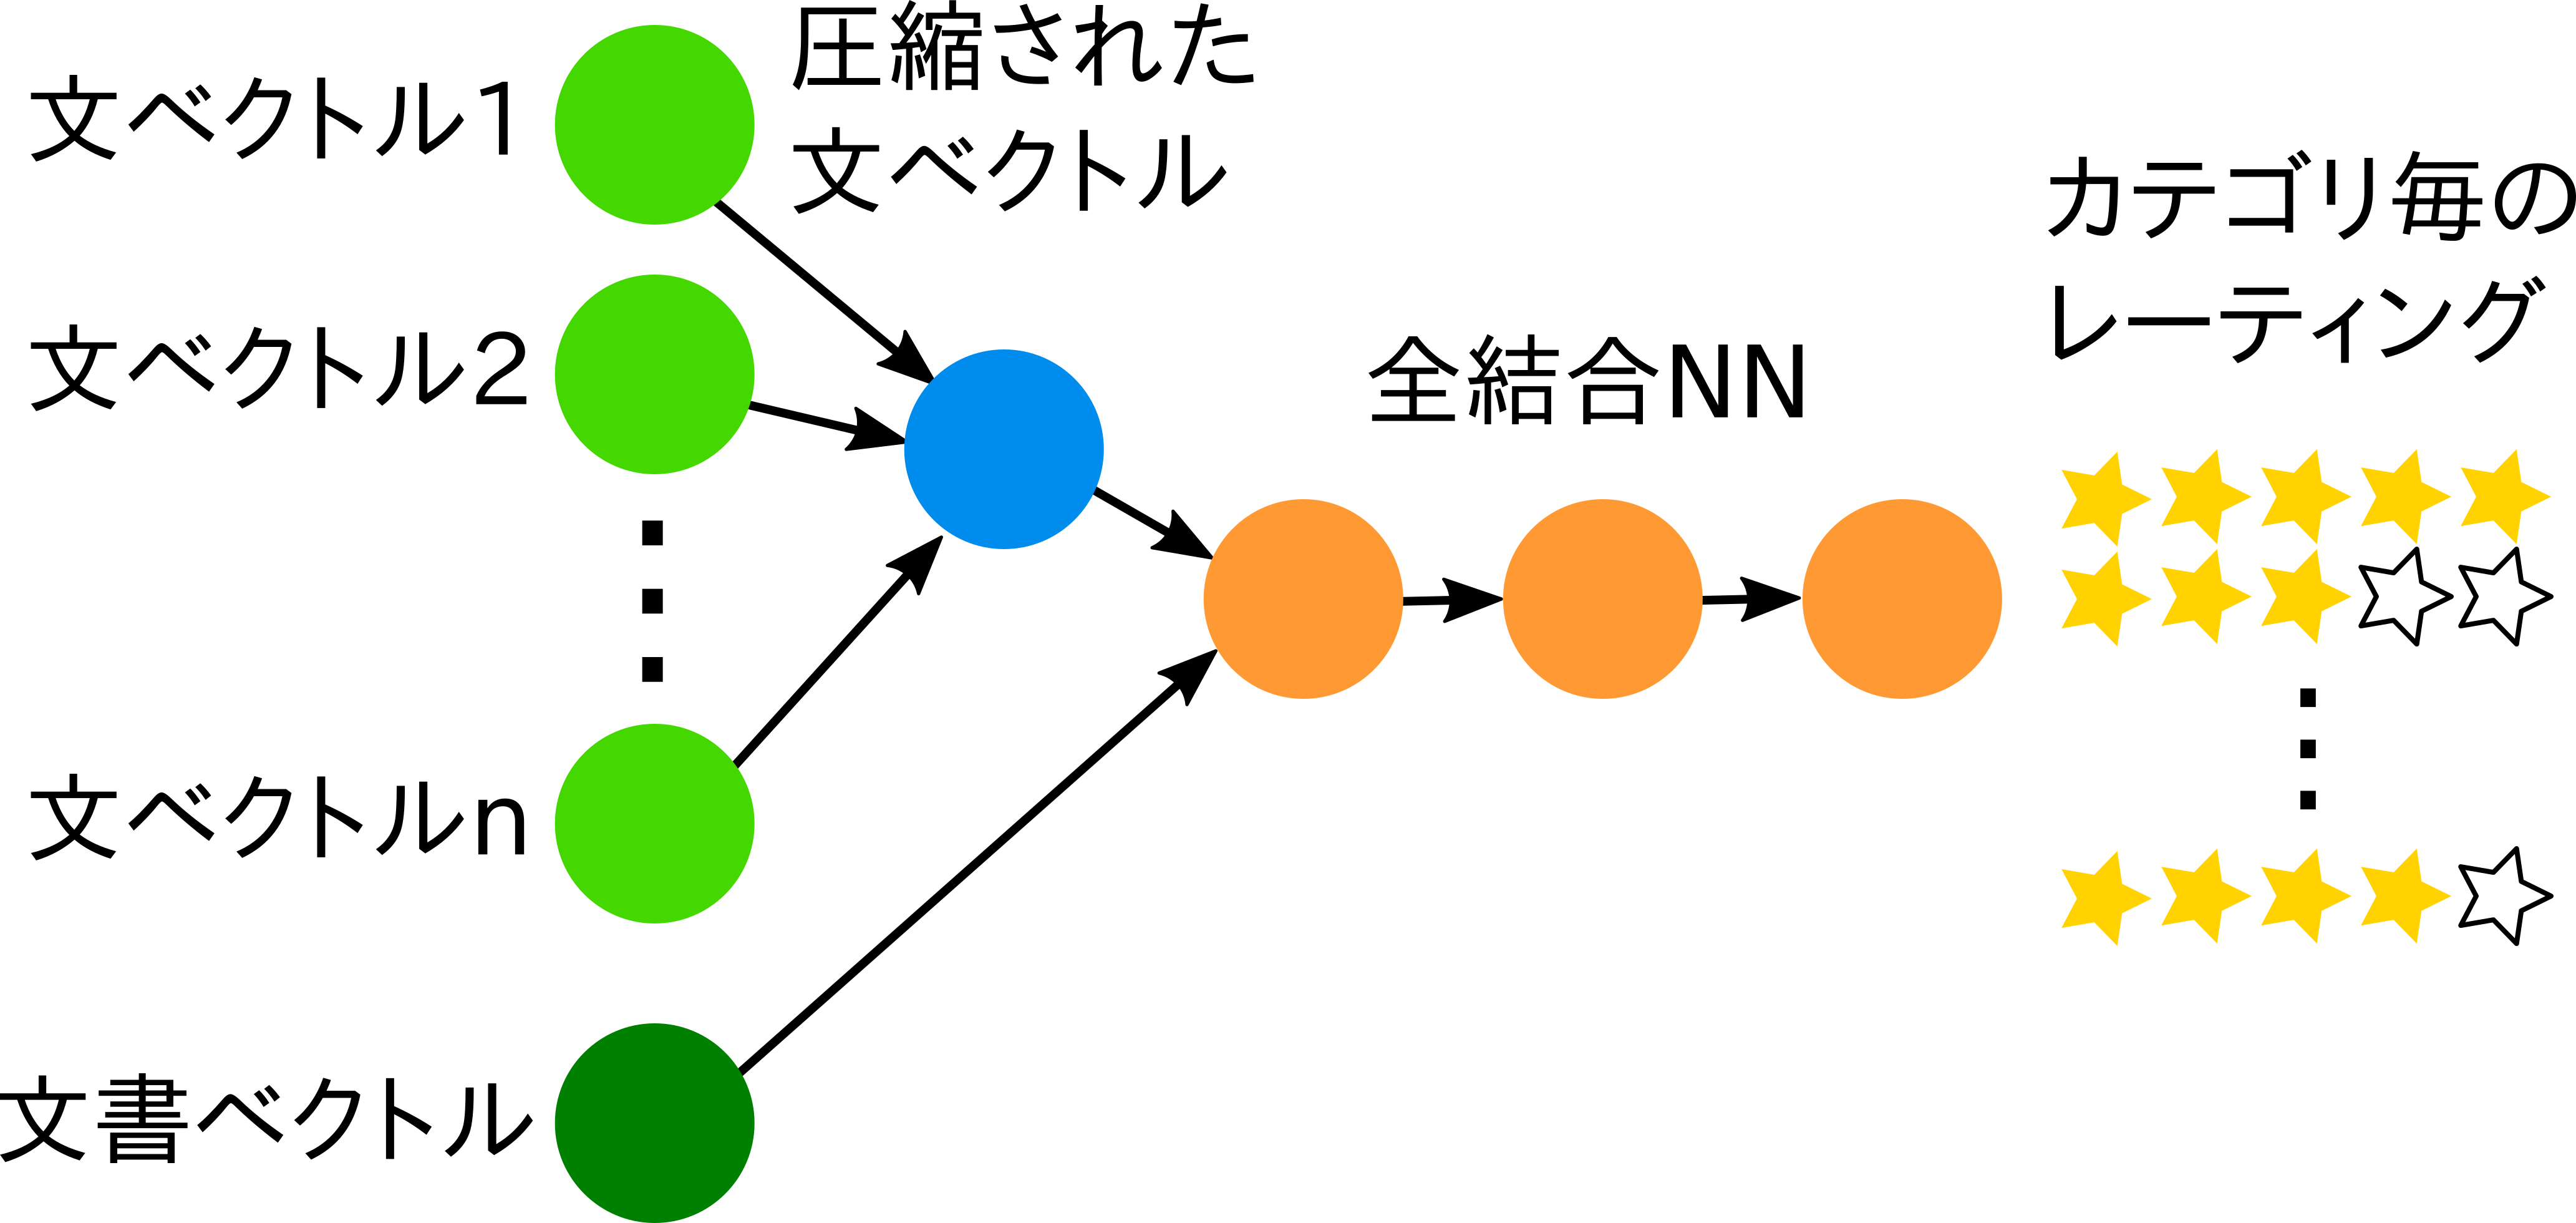
\includegraphics{fig/model.png}
  \caption{全結合ニューラルネットワークによる分類器}
  \label{fig:MyModel}
\end{figure}




提案手法に加え、基準手法としてNNへの入力となる特徴量が異なる4つの手法を用いた。
各手法に用いた特徴量を表\ref{tab:MethodFeatures}に列挙する。

\begin{table}
  \caption{各基準手法に用いられる特徴量}
  \begin{tabular}{l | l}\label{tab:MethodFeatures}
    手法 & 特徴量 \\
    \hline
    基準手法  & レビュー全体の文書ベクトル \\
    提案手法1 & レビュー内で平均した文ベクトル \\
    提案手法2 & レビュー内で重み付け平均によって圧縮された文ベクトル \\
    提案手法3 & レビュー全体の文書ベクトル、
        レビュー内で重み付け平均によって圧縮された文ベクトル \\
  \end{tabular}
\end{table}

提案手法1と提案手法2の比較によって、
文の位置関係が分類に対して重要であるかが示される。
提案手法2と提案手法3の基準手法の比較によって、
文書ベクトルに加え文ベクトルを用いることが有効であるかが示される。


\section{実験}

基準手法及び提案手法について分類精度を測定するために実験を行った。


\subsection{実験設定}

 実験は、分類精度を測定するものと、
その実験で最も精度の高かった提案手法における予測レーティングと
回答レーティングの平均二乗誤差を測定するものの2つを行った。
 分類精度を測定する実験では、1つの基準手法及び3つの提案手法を
それぞれ同じデータセットに適用し、各手法の精度を測定した。
データセットとしては、先行研究\cite{fujitani15}と同様に、
ホテル予約サイト楽天トラベルにおけるレビュー337,266件から
訓練データ300,000件、開発データ10,000件、評価データ10,000件を用いた。
 レーティングの平均二乗誤差を測定する実験は、上記の分類精度を測定する
実験で得られた予測レーティングを用いて測定を行った。
 表\ref{tab:ParametersOfBaselineMethod}と表\ref{tab:ParametersOfMyMethod1}、
表\ref{tab:ParametersOfMyMethod2}、表\ref{tab:ParametersOfMyMethod3}に
各手法でのパラメータ設定を示す。

\begin{table}
  \caption{基準手法のパラメータ設定}
  \begin{tabular}{l | r}\label{tab:ParametersOfBaselineMethod}
    項目 & 値 \\
    \hline
    学習する単語の範囲 & 前後3単語 \\
    単語の最少出現回数 & 5 \\
    ベクトルの次元数 & 600 \\
    中間層の数 & 1 \\
    中間層でのニューロン数 & 512 \\
    入力層及び中間層でのドロップアウト率 & 0.2, 0.5 \\
  \end{tabular}
\end{table}

\begin{table}
  \caption{提案手法1のパラメータ設定}
  \begin{tabular}{l | r}\label{tab:ParametersOfMyMethod1}
    項目 & 値 \\
    \hline
    学習する単語の範囲 & 前後3単語 \\
    単語の最少出現回数 & 5 \\
    ベクトルの次元数 & 600 \\
    中間層の数 & 1 \\
    中間層でのニューロン数 & 512 \\
    入力層及び中間層でのドロップアウト率 & 0.2, 0.5 \\
  \end{tabular}
\end{table}

\begin{table}
  \caption{提案手法2のパラメータ設定}
  \begin{tabular}{l | r}\label{tab:ParametersOfMyMethod2}
    項目 & 値 \\
    \hline
    学習する単語の範囲 & 前後3単語 \\
    単語の最少出現回数 & 5 \\
    ベクトルの次元数 & 600 \\
    中間層の数 & 1 \\
    中間層でのニューロン数 & 512 \\
    入力層及び中間層でのドロップアウト率 & 0.2, 0.5 \\
  \end{tabular}
\end{table}

\begin{table}
  \caption{提案手法3のパラメータ設定}
  \begin{tabular}{l | r}\label{tab:ParametersOfMyMethod3}
    項目 & 値 \\
    \hline
    学習する単語の範囲 & 前後3単語 \\
    単語の最少出現回数 & 5 \\
    ベクトルの次元数 & 600 \\
    中間層の数 & 1 \\
    中間層でのニューロン数 & 512 \\
    入力層及び中間層でのドロップアウト率 & 0.2, 0.5 \\
  \end{tabular}
\end{table}


\subsection{結果}

表\ref{tab:Accuracies}に分類精度を測定する実験の実験結果を示す。

\begin{table}
  \caption{各種法における分類精度}
  \begin{tabular}{l | r}\label{tab:Accuracies}
    手法 & 精度 \\
    \hline
    基準手法 & 0 \\
    提案手法1 & 0 \\
    提案手法2 & 0 \\
    提案手法3 & 0 \\
  \end{tabular}
\end{table}

\subsection{考察}

表\ref{tab:Accuracies}より、



\section{結論}

本研究では、レビュー全体の文書の分散表現に加え、
レビュー内の各文ベクトルに対する分散表現の重み付き平均を用いた
評判分類の手法を提案した。

実験により、従来手法\cite{fujitani15}及びレビュー全体の文書ベクトルのみを
用いた手法に比べ、提案手法が高い分類精度を示すことが分かった。
同時に、これはレビュー内の文の並びが評判分類に重要であることを示す。



\subsection{今後の課題}

今後の課題は、2つに分かれているモデルの統一である。

提案手法は、分類すべき文書とそれが含む文の分散表現を生成する段階、及び、
それらを用いて分類を行う段階の2つの段階に分かれている。
このことは、問題を2つに分けることで個々の問題を単純にしているが、
同時に一つずつ文書の分類を行うことを難しくしている。
また、提案手法において、文書や文の分散表現を事前に生成するための
パラグラフベクトルの手法におけるパラメータは、
実際には最大の分類精度を達成するため分類器のパラメータとして最適化されることが
望ましい。

今後は、これらの問題を解決するために、文書や文の分散表現を生成する過程を
ニューラルネットワークによる分類器に取り込む。
これによって、学習方法の柔軟性を高めると共にさらなる分類精度の向上を目指す。




\begin{thebibliography}{9}
\bibitem{fujitani15}
  藤谷宣典ら,
  隠れ状態を用いたホテルレビューのレーティング予測.
  言語処理学会第21回年次大会, 2015.
\bibitem{quoc14}
  Quoc Le, and Tomas Mikolov,
  Distributed Representations of Sentences and Documents.
  ICML 2014, 2014.
\bibitem{nal14}
  Nal Kalchbrenner, Edward Grefenstette, and Phil Blunsom,
  A Convolutional Neural Network for Modelling Sentences.
  ACL 2014, 2014.
\bibitem{rie14}
  Rie Johnson, and Tong Zhang,
  Effective Use of Word Order for Text Categorization
  with Convolutional Neural Networks.
  NAACL 2015, 2015.
\bibitem{duyu15}
  Duyu Tang, Bing Qin, and Ting Liu,
  Learning Semantic Representation of Users and Products
  for Document Level Sentiment Classification.
  ACL 2015, 2015.
\end{thebibliography}

\end{document}
